%___________________________________________
% parábolas
%___________________________________________

\subsubsection{ Parábola I}
\begin{figure}[H]
  \centering
  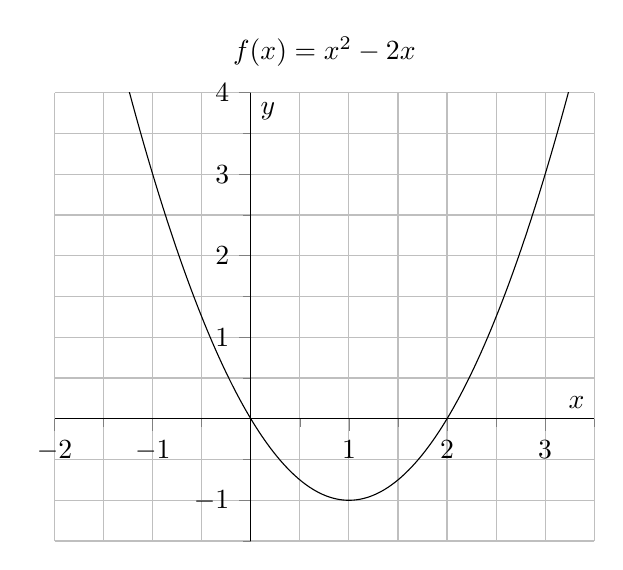
\begin{tikzpicture}
    \begin{axis}[
      xmin=-2, xmax=3.5,
      ymin=-1.5, ymax=4,
      axis x line=middle,
      axis y line=middle,
      axis line style={-},
      tick align=outside,
      grid=both,
      minor tick num=1,
      xlabel={$x$},
      ylabel={$y$},
      title={$f(x)=x^2-2x$}
    ]
      \addplot[domain=-3:4, samples=200] {x^2-2*x};
    \end{axis}
  \end{tikzpicture}
  \caption{Parábola $f(x)=x^2-2x$.}
\end{figure}

%---------------------------------
%Parábola II
%---------------------------------

\subsubsection{ Parábola II}
\begin{figure}[H]
  \centering
  \begin{tikzpicture}
    \begin{axis}[
      xmin=-1, xmax=3,
      ymin=-1.5, ymax=1.5,
      axis x line=middle,
      axis y line=middle,
      axis line style={-},
      tick align=outside,
      %grid=both,
      minor tick num=1,
      xlabel={$x$},
      ylabel={$y$},
      title={$f(x)=x^2-2x$}
    ]
      \addplot[domain=-3:4, samples=200] {-x^2+2*x};
      %\draw[line width=0.6pt] (1,0) -- (1,1);
      %\draw[line width=0.6pt] (2.5,0) -- (2.,-1.5);
    \end{axis}
  \end{tikzpicture}
  \caption{Parábola $f(x)=x^2-2x$.}
\end{figure}

%--------------------------
% Parábola 3 
%--------------------------
\subsubsection{ Parábola III}

\begin{figure}[H]
  \centering
  \begin{tikzpicture}
    \begin{axis}[
      xmin=-.5, xmax=3,
      ymin=-1.1, ymax=1.5,
      axis x line=middle,
      axis y line=middle,
      axis line style={-},
      tick align=outside,
      %grid=both,
      minor tick num=1,
      xlabel={$x$},
      ylabel={$y$},
      title={$f(x)=x^2-2x$}
    ]
      \addplot[domain=-.5:2.5, samples=200] {x^2-2*x};
      %\draw[line width=0.6pt] (1,0) -- (1,1);
      %\draw[line width=0.6pt] (2.5,0) -- (2.,-1.5);
    \end{axis}
  \end{tikzpicture}
  \caption{Parábola $f(x)=x^2-2x$.}
\end{figure}